\documentclass[]{book}
\usepackage{lmodern}
\usepackage{amssymb,amsmath}
\usepackage{ifxetex,ifluatex}
\usepackage{fixltx2e} % provides \textsubscript
\ifnum 0\ifxetex 1\fi\ifluatex 1\fi=0 % if pdftex
  \usepackage[T1]{fontenc}
  \usepackage[utf8]{inputenc}
\else % if luatex or xelatex
  \ifxetex
    \usepackage{mathspec}
  \else
    \usepackage{fontspec}
  \fi
  \defaultfontfeatures{Ligatures=TeX,Scale=MatchLowercase}
\fi
% use upquote if available, for straight quotes in verbatim environments
\IfFileExists{upquote.sty}{\usepackage{upquote}}{}
% use microtype if available
\IfFileExists{microtype.sty}{%
\usepackage{microtype}
\UseMicrotypeSet[protrusion]{basicmath} % disable protrusion for tt fonts
}{}
\usepackage[margin=1in]{geometry}
\usepackage{hyperref}
\hypersetup{unicode=true,
            pdftitle={R, Databases and Docker},
            pdfauthor={M. Edward (Ed) Borasky, editor},
            pdfborder={0 0 0},
            breaklinks=true}
\urlstyle{same}  % don't use monospace font for urls
\usepackage{natbib}
\bibliographystyle{apalike}
\usepackage{color}
\usepackage{fancyvrb}
\newcommand{\VerbBar}{|}
\newcommand{\VERB}{\Verb[commandchars=\\\{\}]}
\DefineVerbatimEnvironment{Highlighting}{Verbatim}{commandchars=\\\{\}}
% Add ',fontsize=\small' for more characters per line
\usepackage{framed}
\definecolor{shadecolor}{RGB}{248,248,248}
\newenvironment{Shaded}{\begin{snugshade}}{\end{snugshade}}
\newcommand{\AlertTok}[1]{\textcolor[rgb]{0.94,0.16,0.16}{#1}}
\newcommand{\AnnotationTok}[1]{\textcolor[rgb]{0.56,0.35,0.01}{\textbf{\textit{#1}}}}
\newcommand{\AttributeTok}[1]{\textcolor[rgb]{0.77,0.63,0.00}{#1}}
\newcommand{\BaseNTok}[1]{\textcolor[rgb]{0.00,0.00,0.81}{#1}}
\newcommand{\BuiltInTok}[1]{#1}
\newcommand{\CharTok}[1]{\textcolor[rgb]{0.31,0.60,0.02}{#1}}
\newcommand{\CommentTok}[1]{\textcolor[rgb]{0.56,0.35,0.01}{\textit{#1}}}
\newcommand{\CommentVarTok}[1]{\textcolor[rgb]{0.56,0.35,0.01}{\textbf{\textit{#1}}}}
\newcommand{\ConstantTok}[1]{\textcolor[rgb]{0.00,0.00,0.00}{#1}}
\newcommand{\ControlFlowTok}[1]{\textcolor[rgb]{0.13,0.29,0.53}{\textbf{#1}}}
\newcommand{\DataTypeTok}[1]{\textcolor[rgb]{0.13,0.29,0.53}{#1}}
\newcommand{\DecValTok}[1]{\textcolor[rgb]{0.00,0.00,0.81}{#1}}
\newcommand{\DocumentationTok}[1]{\textcolor[rgb]{0.56,0.35,0.01}{\textbf{\textit{#1}}}}
\newcommand{\ErrorTok}[1]{\textcolor[rgb]{0.64,0.00,0.00}{\textbf{#1}}}
\newcommand{\ExtensionTok}[1]{#1}
\newcommand{\FloatTok}[1]{\textcolor[rgb]{0.00,0.00,0.81}{#1}}
\newcommand{\FunctionTok}[1]{\textcolor[rgb]{0.00,0.00,0.00}{#1}}
\newcommand{\ImportTok}[1]{#1}
\newcommand{\InformationTok}[1]{\textcolor[rgb]{0.56,0.35,0.01}{\textbf{\textit{#1}}}}
\newcommand{\KeywordTok}[1]{\textcolor[rgb]{0.13,0.29,0.53}{\textbf{#1}}}
\newcommand{\NormalTok}[1]{#1}
\newcommand{\OperatorTok}[1]{\textcolor[rgb]{0.81,0.36,0.00}{\textbf{#1}}}
\newcommand{\OtherTok}[1]{\textcolor[rgb]{0.56,0.35,0.01}{#1}}
\newcommand{\PreprocessorTok}[1]{\textcolor[rgb]{0.56,0.35,0.01}{\textit{#1}}}
\newcommand{\RegionMarkerTok}[1]{#1}
\newcommand{\SpecialCharTok}[1]{\textcolor[rgb]{0.00,0.00,0.00}{#1}}
\newcommand{\SpecialStringTok}[1]{\textcolor[rgb]{0.31,0.60,0.02}{#1}}
\newcommand{\StringTok}[1]{\textcolor[rgb]{0.31,0.60,0.02}{#1}}
\newcommand{\VariableTok}[1]{\textcolor[rgb]{0.00,0.00,0.00}{#1}}
\newcommand{\VerbatimStringTok}[1]{\textcolor[rgb]{0.31,0.60,0.02}{#1}}
\newcommand{\WarningTok}[1]{\textcolor[rgb]{0.56,0.35,0.01}{\textbf{\textit{#1}}}}
\usepackage{longtable,booktabs}
\usepackage{graphicx,grffile}
\makeatletter
\def\maxwidth{\ifdim\Gin@nat@width>\linewidth\linewidth\else\Gin@nat@width\fi}
\def\maxheight{\ifdim\Gin@nat@height>\textheight\textheight\else\Gin@nat@height\fi}
\makeatother
% Scale images if necessary, so that they will not overflow the page
% margins by default, and it is still possible to overwrite the defaults
% using explicit options in \includegraphics[width, height, ...]{}
\setkeys{Gin}{width=\maxwidth,height=\maxheight,keepaspectratio}
\IfFileExists{parskip.sty}{%
\usepackage{parskip}
}{% else
\setlength{\parindent}{0pt}
\setlength{\parskip}{6pt plus 2pt minus 1pt}
}
\setlength{\emergencystretch}{3em}  % prevent overfull lines
\providecommand{\tightlist}{%
  \setlength{\itemsep}{0pt}\setlength{\parskip}{0pt}}
\setcounter{secnumdepth}{5}
% Redefines (sub)paragraphs to behave more like sections
\ifx\paragraph\undefined\else
\let\oldparagraph\paragraph
\renewcommand{\paragraph}[1]{\oldparagraph{#1}\mbox{}}
\fi
\ifx\subparagraph\undefined\else
\let\oldsubparagraph\subparagraph
\renewcommand{\subparagraph}[1]{\oldsubparagraph{#1}\mbox{}}
\fi

%%% Use protect on footnotes to avoid problems with footnotes in titles
\let\rmarkdownfootnote\footnote%
\def\footnote{\protect\rmarkdownfootnote}

%%% Change title format to be more compact
\usepackage{titling}

% Create subtitle command for use in maketitle
\newcommand{\subtitle}[1]{
  \posttitle{
    \begin{center}\large#1\end{center}
    }
}

\setlength{\droptitle}{-2em}

  \title{R, Databases and Docker}
    \pretitle{\vspace{\droptitle}\centering\huge}
  \posttitle{\par}
    \author{M. Edward (Ed) Borasky, editor}
    \preauthor{\centering\large\emph}
  \postauthor{\par}
      \predate{\centering\large\emph}
  \postdate{\par}
    \date{2018-09-04}

\usepackage{booktabs}

\usepackage{amsthm}
\newtheorem{theorem}{Theorem}[chapter]
\newtheorem{lemma}{Lemma}[chapter]
\theoremstyle{definition}
\newtheorem{definition}{Definition}[chapter]
\newtheorem{corollary}{Corollary}[chapter]
\newtheorem{proposition}{Proposition}[chapter]
\theoremstyle{definition}
\newtheorem{example}{Example}[chapter]
\theoremstyle{definition}
\newtheorem{exercise}{Exercise}[chapter]
\theoremstyle{remark}
\newtheorem*{remark}{Remark}
\newtheorem*{solution}{Solution}
\begin{document}
\maketitle

{
\setcounter{tocdepth}{1}
\tableofcontents
}
\hypertarget{introduction}{%
\chapter{Introduction}\label{introduction}}

\hypertarget{who-are-we}{%
\section{Who are we?}\label{who-are-we}}

\begin{itemize}
\tightlist
\item
  M. Edward (Ed) Borasky
\end{itemize}

\hypertarget{prerequisites}{%
\section{Prerequisites}\label{prerequisites}}

You will need

\begin{itemize}
\tightlist
\item
  A computer running Windows, MacOS, or Linux. Any Linux distro that
  will run Docker Community Edition, R and RStudio will work,
\item
  R, and
\item
  Docker hosting.
\end{itemize}

The database we use is PostgreSQL 10, but you do not need to install
that - it's installed via a Docker image. RStudio 1.2 is highly
recommended but not required.

\hypertarget{miniconda-integration}{%
\chapter{Miniconda Integration}\label{miniconda-integration}}

\hypertarget{why-do-this}{%
\section{Why do this?}\label{why-do-this}}

A number of R deep learning packages use Python under the hood.
RStudio's \textbf{keras} \citep{R-keras} package, for example, works
this way. Also, the R \textbf{docker} \citep{R-docker} package works by
calling a Python Docker API library from R via \textbf{reticulate}
\citep{R-reticulate}. And, of course, you'll probably end up receiving a
Jupyter notebook or two even if you're a die-hard RStudio user.

\href{https://conda.io/miniconda.html}{\texttt{Miniconda}} is a
bare-bones minimalist version of the rather large Anaconda environment.
If you're doing Python data science, you probably have the full Anaconda
installed already. But for R programmers, we only want enough Python for
the R packages that use Python libraries to work. So \ldots{} here we
go!

\hypertarget{install-the-installr-package.}{%
\section{\texorpdfstring{Install the \texttt{installr}
package.}{Install the installr package.}}\label{install-the-installr-package.}}

There's an R package called \textbf{installr} \citep{R-installr} that
can download and run a Windows installer.

\begin{Shaded}
\begin{Highlighting}[]
\ControlFlowTok{if}\NormalTok{ (}\OperatorTok{!}\KeywordTok{require}\NormalTok{(installr)) }\KeywordTok{install.packages}\NormalTok{(}\StringTok{"installr"}\NormalTok{)}
\KeywordTok{library}\NormalTok{(installr)}
\end{Highlighting}
\end{Shaded}

\hypertarget{install-miniconda3}{%
\section{\texorpdfstring{Install
\texttt{Miniconda3}}{Install Miniconda3}}\label{install-miniconda3}}

The following R code chunk will download and install
\texttt{Miniconda3}.

\begin{Shaded}
\begin{Highlighting}[]
\KeywordTok{install.URL}\NormalTok{(}\StringTok{"https://repo.continuum.io/miniconda/Miniconda3-latest-Windows-x86_64.exe"}\NormalTok{)}
\end{Highlighting}
\end{Shaded}

Here are the screenshots you'll see:

\begin{center}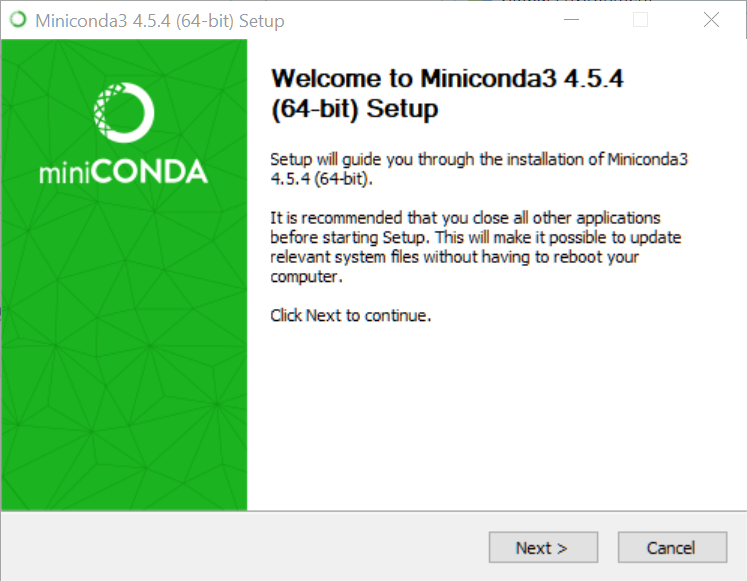
\includegraphics[width=0.9\linewidth]{screenshots/2018-08-31_16_12_57-Miniconda3_4.5.4_(64-bit)_Setup} \end{center}

Click \texttt{Next}.

\begin{center}\rule{0.5\linewidth}{\linethickness}\end{center}

\begin{center}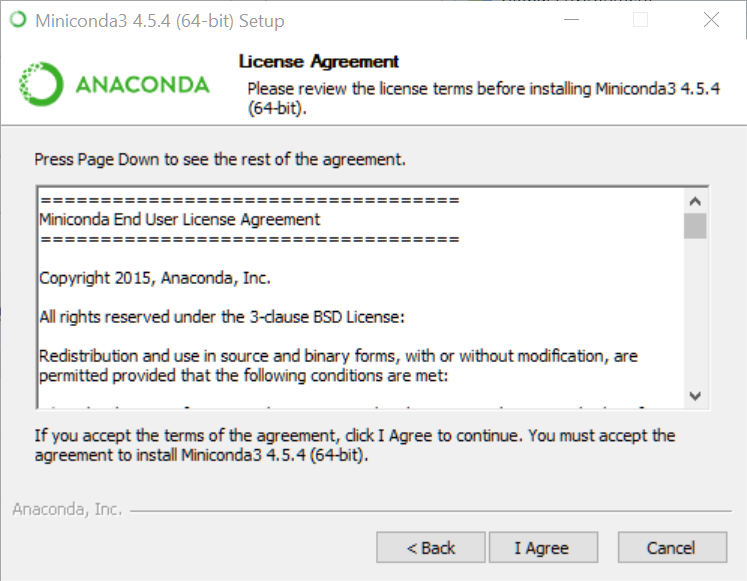
\includegraphics[width=0.9\linewidth]{screenshots/2018-08-31_16_13_57-Miniconda3_4.5.4_(64-bit)_Setup} \end{center}

Click \texttt{I\ Agree}.

\begin{center}\rule{0.5\linewidth}{\linethickness}\end{center}

\begin{center}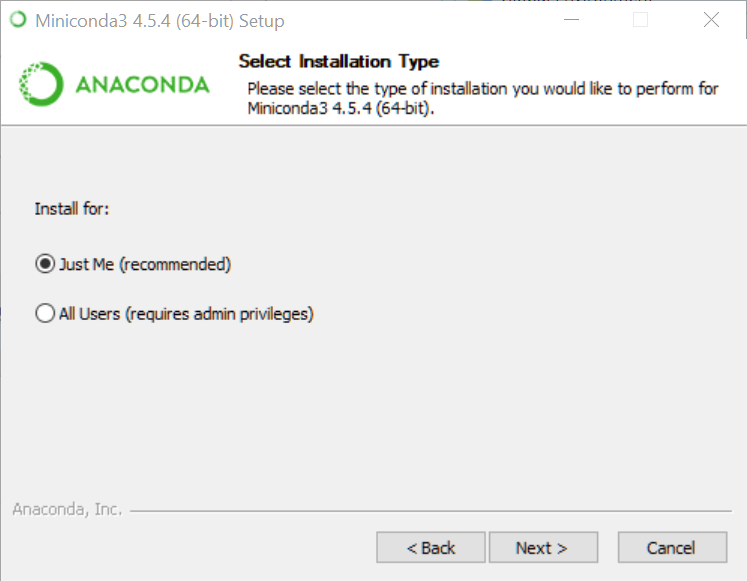
\includegraphics[width=0.9\linewidth]{screenshots/2018-08-31_16_14_23-Miniconda3_4.5.4_(64-bit)_Setup} \end{center}

\texttt{Just\ Me}, \texttt{Next}.

\begin{center}\rule{0.5\linewidth}{\linethickness}\end{center}

\begin{center}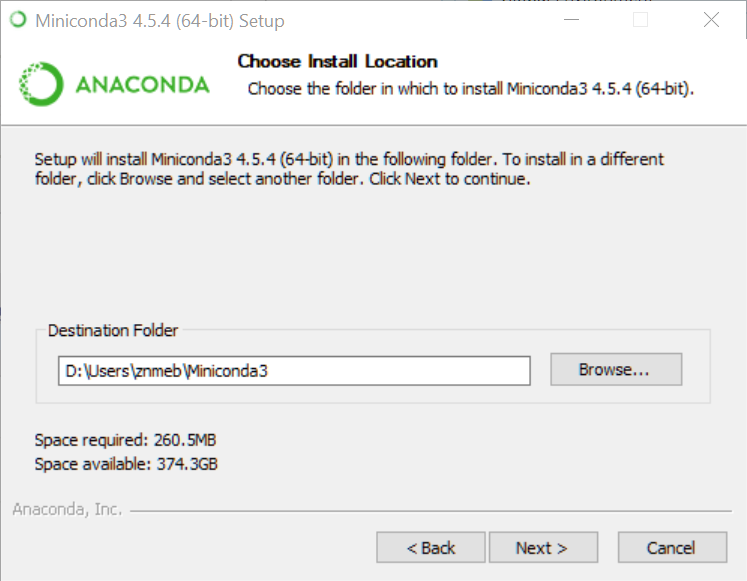
\includegraphics[width=0.9\linewidth]{screenshots/2018-08-31_16_16_11-Miniconda3_4.5.4_(64-bit)_Setup} \end{center}

Choose the install location. The default is your home directory, which
on my laptop is a small SSD. So I changed it to the \texttt{D} drive,
which is a terabyte spinning disk. After you've set the install
location, click \texttt{Next}.

\begin{center}\rule{0.5\linewidth}{\linethickness}\end{center}

\begin{center}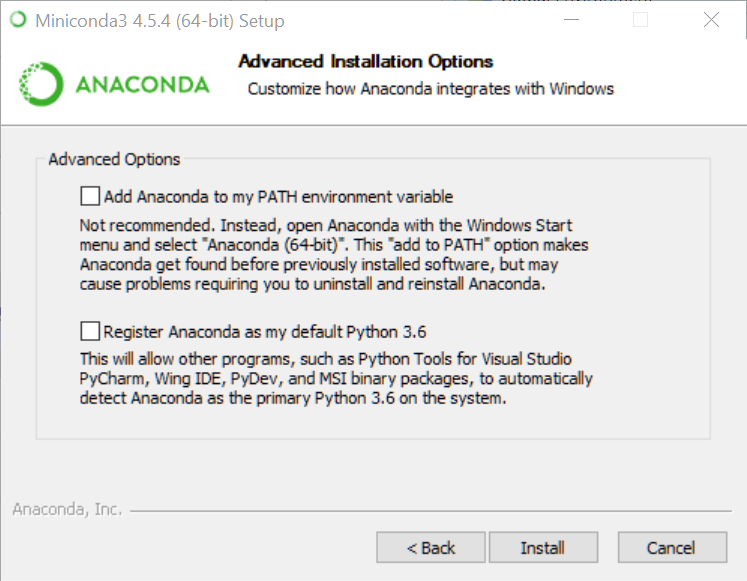
\includegraphics[width=0.9\linewidth]{screenshots/2018-08-31_16_18_47-Miniconda3_4.5.4_(64-bit)_Setup} \end{center}

Clear both check boxes and click \texttt{Install}.

\begin{center}\rule{0.5\linewidth}{\linethickness}\end{center}

\begin{center}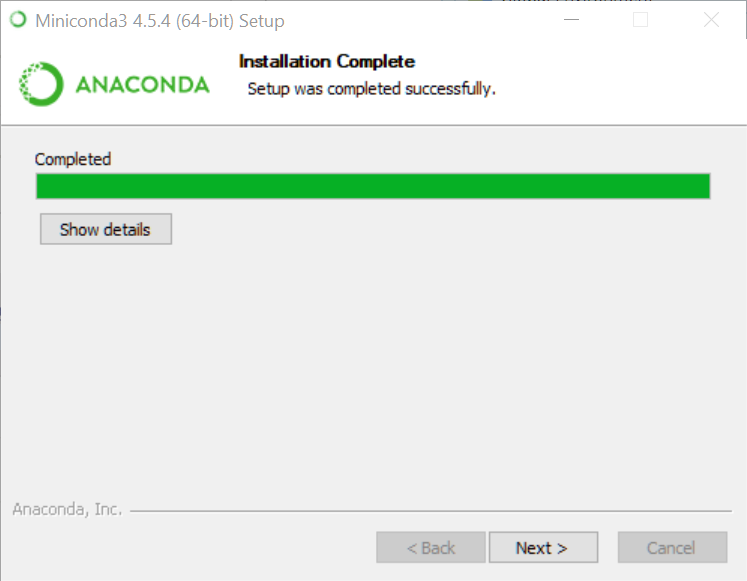
\includegraphics[width=0.9\linewidth]{screenshots/2018-08-31_16_21_12-Miniconda3_4.5.4_(64-bit)_Setup} \end{center}

Click \texttt{Next}.

\begin{center}\rule{0.5\linewidth}{\linethickness}\end{center}

\begin{center}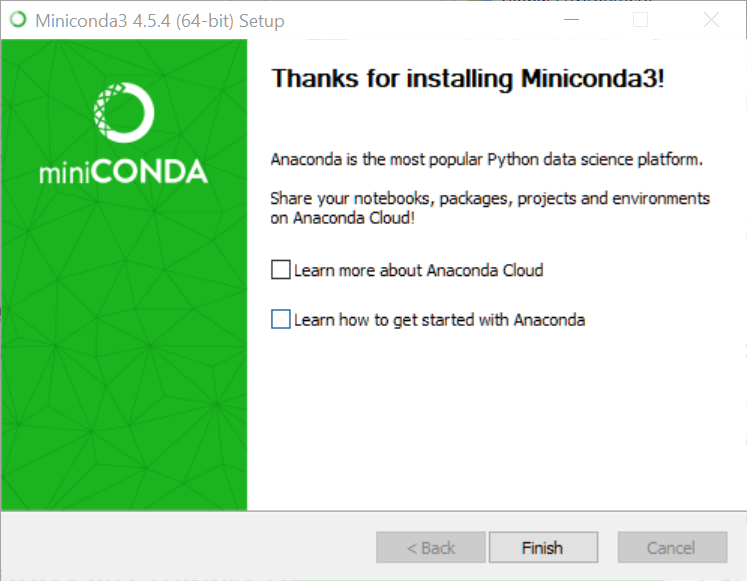
\includegraphics[width=0.9\linewidth]{screenshots/2018-08-31_16_21_44-Miniconda3_4.5.4_(64-bit)_Setup} \end{center}

Clear the check boxes and click \texttt{Finish}.

\hypertarget{install-reticulate}{%
\section{\texorpdfstring{Install
\texttt{reticulate}}{Install reticulate}}\label{install-reticulate}}

\begin{Shaded}
\begin{Highlighting}[]
\ControlFlowTok{if}\NormalTok{ (}\OperatorTok{!}\KeywordTok{require}\NormalTok{(reticulate)) }\KeywordTok{install.packages}\NormalTok{(}\StringTok{"reticulate"}\NormalTok{)}
\KeywordTok{library}\NormalTok{(reticulate)}
\end{Highlighting}
\end{Shaded}

Did it work?

\begin{Shaded}
\begin{Highlighting}[]
\KeywordTok{py_discover_config}\NormalTok{()}
\end{Highlighting}
\end{Shaded}

\begin{verbatim}
## python:         /usr/bin/python
## libpython:      /usr/lib/libpython3.7m.so
## pythonhome:     /usr:/usr
## version:        3.7.0 (default, Jul 15 2018, 10:44:58)  [GCC 8.1.1 20180531]
## numpy:          /usr/lib/python3.7/site-packages/numpy
## numpy_version:  1.15.1
## 
## python versions found: 
##  /home/znmeb/.conda/envs/docker/bin/python
##  /usr/bin/python
##  /usr/bin/python3
\end{verbatim}

\hypertarget{docker-hosting-for-windows}{%
\chapter{Docker Hosting for Windows}\label{docker-hosting-for-windows}}

\hypertarget{hardware-requirements}{%
\section{Hardware requirements}\label{hardware-requirements}}

You will need an Intel or AMD processor with 64-bit hardware and the
hardware virtualization feature. Most machines you buy today will have
that, but older ones may not. You will need to go into the BIOS /
firmware and enable the virtualization feature. You will need at least 4
gigabytes of RAM!

\hypertarget{software-requirements}{%
\section{Software requirements}\label{software-requirements}}

You will need Windows 7 64-bit or later. If you can afford it, I highly
recommend upgrading to Windows 10 Pro.

\hypertarget{windows-7-8-8.1-and-windows-10-home-64-bit}{%
\subsection{Windows 7, 8, 8.1 and Windows 10 Home (64
bit)}\label{windows-7-8-8.1-and-windows-10-home-64-bit}}

Install Docker Toolbox. The instructions are here:
\url{https://docs.docker.com/toolbox/toolbox_install_windows/}. Make
sure you try the test cases and they work!

\hypertarget{windows-10-pro}{%
\subsection{Windows 10 Pro}\label{windows-10-pro}}

Install Docker for Windows \emph{stable}. The instructions are here:
\url{https://docs.docker.com/docker-for-windows/install/\#start-docker-for-windows}.
Again, make sure you try the test cases and they work.

\hypertarget{docker-for-windows-settings}{%
\section{Docker for Windows
settings}\label{docker-for-windows-settings}}

\hypertarget{shared-drives}{%
\subsection{Shared drives}\label{shared-drives}}

If you're going to mount host files into container filesystems, you need
to set up shared drives. Open the Docker settings dialog and select
\texttt{Shared\ Drives}. Check the drives you want to share. In this
screenshot, the \texttt{D:} drive is my 1 terabyte hard drive.

\begin{center}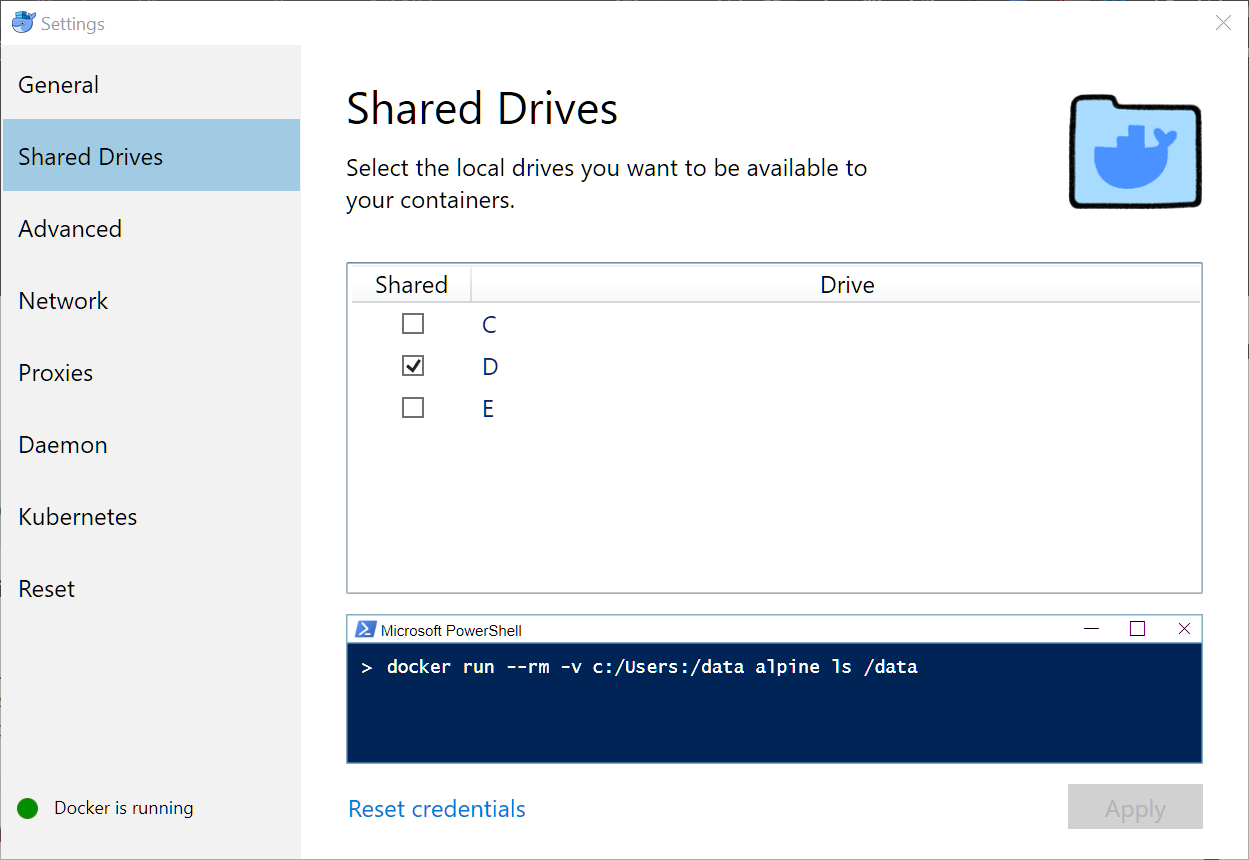
\includegraphics[width=0.9\linewidth]{screenshots/2018-08-26_15_16_51-Shared_Drives} \end{center}

\hypertarget{kubernetes}{%
\subsection{Kubernetes}\label{kubernetes}}

Kubernetes is a container orchestration / cloud management package
that's a major DevOps tool. It's heavily supported by Red Hat and
Google, and as a result is becoming a required skill for DevOps.

However, it's overkill for this project at the moment, and it doesn't
seem to be compatible with the Docker Compose we're using. So you should
make sure it's not enabled.

Go to the \texttt{Kubernetes} dialog and make sure the
\texttt{Enable\ Kubernetes} checkbox is cleared.

\begin{center}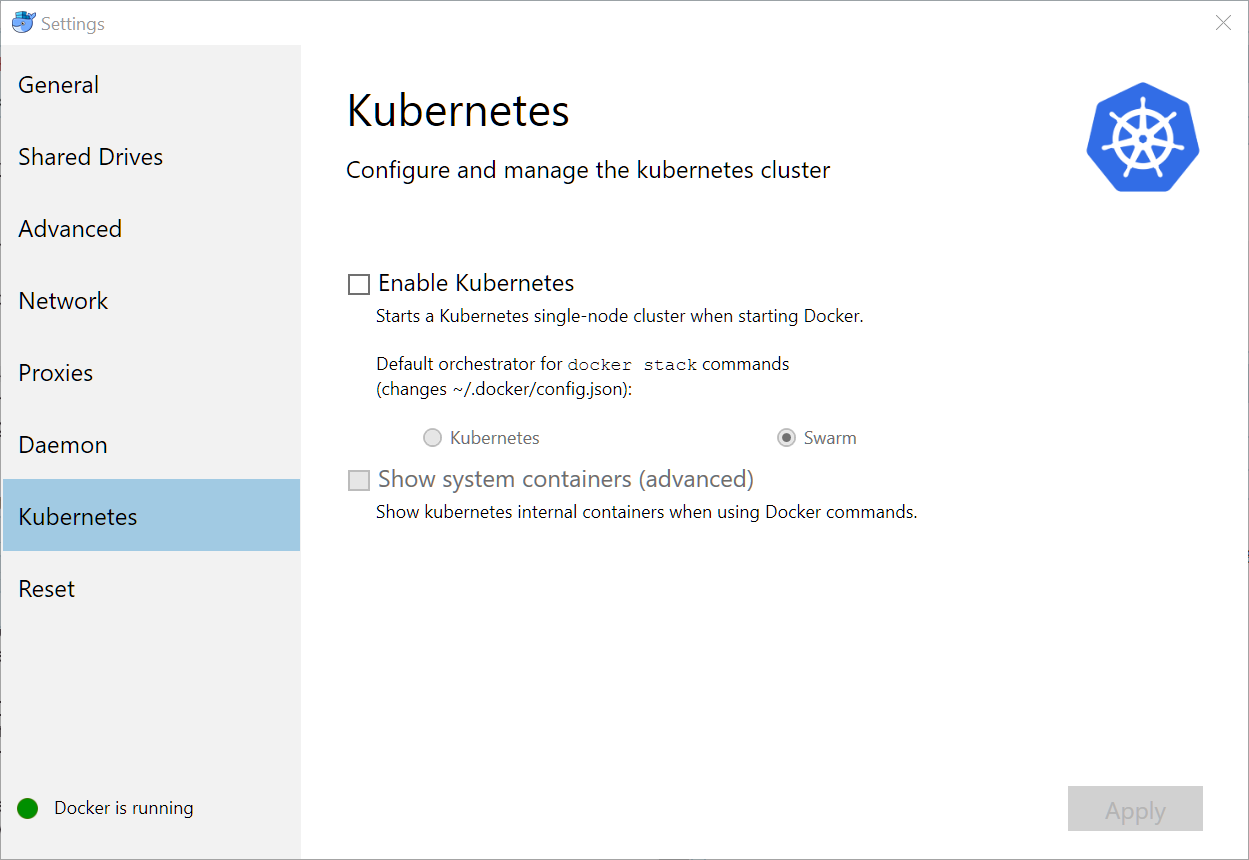
\includegraphics[width=0.9\linewidth]{screenshots/2018-08-26_15_26_22-Kubernetes} \end{center}

\hypertarget{git-github-and-line-endings}{%
\section{Git, GitHub and line
endings}\label{git-github-and-line-endings}}

Git was originally developed for Linux - in fact, it was created by
Linus Torvalds to manage hundreds of different versions of the Linux
kernel on different machines all around the world. As usage has grown,
it's achieved a huge following and is the version control system used by
most large open source projects.

If you're on Windows, there are some things about Git and GitHub you
need to watch. First of all, there are quite a few tools for running Git
on Windows, but the RStudio default and recommended one is Git for
Windows (\url{https://git-scm.com/download/win}).

By default, text files on Linux end with a single linefeed
(\texttt{\textbackslash{}n}) character. But on Windows, text files end
with a carriage return and a line feed
(\texttt{\textbackslash{}r\textbackslash{}n}). See
\url{https://en.wikipedia.org/wiki/Newline} for the gory details.

Git defaults to checking files out in the native mode. So if you're on
Linux, a text file will show up with the Linux convention, and if you're
on Windows, it will show up with the Windows convention.

Most of the time this doesn't cause any problems. But Docker containers
usually run Linux, and if you have files from a repository on Windows
that you've sent to the container, the container may malfunction or give
weird results.

In particular, executable \texttt{sh} or \texttt{bash} scripts will fail
in a Docker container if they have Windows line endings. You may see an
error message with \texttt{\textbackslash{}r} in it, which means the
shell saw the carriage return (\texttt{\textbackslash{}r}) and gave up.
But often you'll see no hint at all what the problem was.

So you need a way to tell Git that some files need to be checked out
with Linux line endings. See
\url{https://help.github.com/articles/dealing-with-line-endings/} for
the details. Summary:

\begin{enumerate}
\def\labelenumi{\arabic{enumi}.}
\tightlist
\item
  You'll need a \texttt{.gitattributes} file in the root of the
  repository.
\item
  In that file, all text files (scripts, program source, data, etc.)
  that are destined for a Docker container will need to have the
  designator \texttt{\textless{}spec\textgreater{}\ text\ eol=lf}, where
  \texttt{\textless{}spec\textgreater{}} is the file name specifier, for
  example, \texttt{*.sh}.
\end{enumerate}

\hypertarget{installing-the-r-docker-package}{%
\section{\texorpdfstring{Installing the R
\href{https://bhaskarvk.github.io/docker/}{\texttt{docker}}
package}{Installing the R docker package}}\label{installing-the-r-docker-package}}

First, if you haven't already, install Miniconda3 and
\texttt{reticulate}. The instructions are in
\protect\hyperlink{miniconda-installation}{Chapter 1}.

Now, install the R \texttt{docker} package:

\begin{Shaded}
\begin{Highlighting}[]
\ControlFlowTok{if}\NormalTok{ (}\OperatorTok{!}\KeywordTok{require}\NormalTok{(docker)) }\KeywordTok{install.packages}\NormalTok{(}\StringTok{"docker"}\NormalTok{)}
\KeywordTok{library}\NormalTok{(docker)}
\end{Highlighting}
\end{Shaded}

Create a \texttt{conda} virtual environment:

\begin{Shaded}
\begin{Highlighting}[]
\KeywordTok{library}\NormalTok{(reticulate)}
\KeywordTok{conda_remove}\NormalTok{(}\DataTypeTok{envname =} \StringTok{"docker"}\NormalTok{)}
\KeywordTok{conda_create}\NormalTok{(}\DataTypeTok{envname =} \StringTok{"docker"}\NormalTok{)}
\KeywordTok{conda_install}\NormalTok{(}\DataTypeTok{envname =} \StringTok{"docker"}\NormalTok{, }\DataTypeTok{packages =} \StringTok{"docker"}\NormalTok{, }\DataTypeTok{pip =} \OtherTok{TRUE}\NormalTok{)}
\KeywordTok{use_condaenv}\NormalTok{(}\StringTok{"docker"}\NormalTok{)}
\end{Highlighting}
\end{Shaded}

Did it work?

\begin{Shaded}
\begin{Highlighting}[]
\KeywordTok{library}\NormalTok{(docker)}
\NormalTok{client <-}\StringTok{ }\NormalTok{docker}\OperatorTok{$}\KeywordTok{from_env}\NormalTok{()}
\NormalTok{s <-}\StringTok{ }\NormalTok{client}\OperatorTok{$}\NormalTok{containers}\OperatorTok{$}\KeywordTok{run}\NormalTok{(}\StringTok{"alpine"}\NormalTok{, }\StringTok{'echo -n "Hello World!"'}\NormalTok{, }\DataTypeTok{remove=}\OtherTok{TRUE}\NormalTok{)}
\KeywordTok{print}\NormalTok{(s}\OperatorTok{$}\KeywordTok{decode}\NormalTok{(}\StringTok{"UTF-8"}\NormalTok{))}
\end{Highlighting}
\end{Shaded}

\begin{verbatim}
## [1] "Hello World!"
\end{verbatim}

\bibliography{book.bib,packages.bib}


\end{document}
